\documentclass[10pt,letterpaper]{amspset}
\usepackage{fullpage}
\usepackage{gensymb}
\usepackage{graphicx}
\usepackage{tikz}
\usepackage{amsmath}
\usepackage{pgfplots}
\graphicspath{ {./images/} }
\notag

% info for header block in upper right hand corner
\name{Brady Lamson}
\class{MATH 1120 SPRING 2021}
\assignment{Graphing Trig Functions}
\duedate{Always earlier than I would like}

\begin{document}

Multiplying a trig function by a constant value will change the graph.

Consider the function $a sin \theta$. Then $|a|$ is called the \underline{amplitude} of the function. \medskip

In terms of the graph of $a sin \theta$, the amplitude is half the vertical distance between the highest point on the graph and the lowest point on the graph. \medskip

This means that $tan \theta$, $cot \theta$, $sec \theta$ and $csc \theta$ do not have an amplitude. Such graphs do not have a highest or lowest points. This makes sense as they all have a range that dabbles in infinity. \medskip

Now, we CAN manipulate those functions in the same way. It just isn't referred to as the amplitude. \medskip





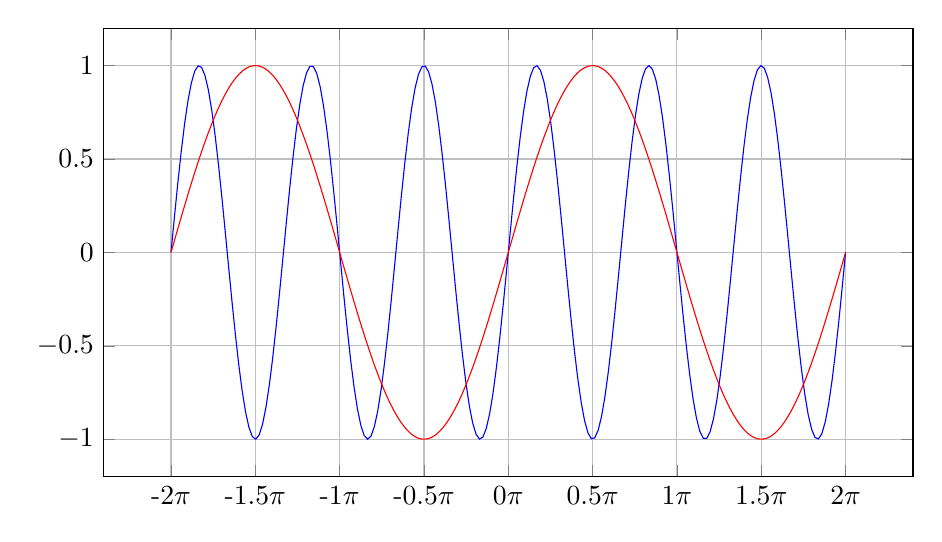
\begin{tikzpicture}
\begin{axis}
[
% This is an example sine graph! This will be useful later.
grid=both,
domain=-2*pi:2*pi,
samples=200,
no marks,
xticklabels={-2$\pi$,-1.5$\pi$,...$\pi$,2$\pi$},
xtick={-6.2832,-4.7124,...,6.2832},
x post scale=1.5
]
\addplot {sin(deg(3*x))};
\addplot {sin(deg(x))};
\end{axis}
\end{tikzpicture}

\end{document}